% \documentclass[preprint,12pt]{elsarticle}
\documentclass[preprint,review,12pt]{elsarticle}
% \documentclass[final,1p,times]{elsarticle}
%% \documentclass[final,1p,times,twocolumn]{elsarticle}
% \documentclass[final,3p,times]{elsarticle}
%% \documentclass[final,3p,times,twocolumn]{elsarticle}
% \documentclass[final,5p,times]{elsarticle}
% \documentclass[final,5p,times,twocolumn]{elsarticle}

\usepackage{graphicx}
\usepackage{amssymb}
\usepackage{lineno}
\usepackage[T1]{fontenc}
\usepackage[utf8]{inputenc}
\usepackage{natbib}
\usepackage{float}

\journal{Applied Ergonomics}

\begin{document}

    % TODO
    %  - cover letter
    %  - fig

    \begin{frontmatter}

        \title{Sex differences in upper limb musculoskeletal biomechanics during a lifting task}

        %% use the tnoteref command within \title for footnotes;
        %% use the tnotetext command for the associated footnote;
        %% use the fnref command within \author or \address for footnotes;
        %% use the fntext command for the associated footnote;
        %% use the corref command within \author for corresponding author footnotes;
        %% use the cortext command for the associated footnote;
        %% use the ead command for the email address,
        %% and the form \ead[url] for the home page:
        %%
        %% \title{Title\tnoteref{label1}}
        %% \tnotetext[label1]{}
        %% \author{Name\corref{cor1}\fnref{label2}}
        %% \ead{email address}
        %% \ead[url]{home page}
        %% \fntext[label2]{}
        %% \cortext[cor1]{}
        %% \address{Address\fnref{label3}}
        %% \fntext[label3]{}

        \author[1]{Martinez Romain\corref{cor1}}
        \ead{martinez.staps@gmail.com}
        \author[1]{Assila Najoua}
        \author[1]{Goubault Etienne}
        \author[1]{Begon Mickaël}

        \address[1]{School of Kinesiology and Exercise Science, Faculty of Medicine, University of Montreal}

        \cortext[cor1]{corresponding author.}


        \begin{abstract}
            Women experience higher prevalence of work-related upper limb musculoskeletal disorders compared to men.
            Previous studies have investigated the biological, kinematic and electromyographic sex-related differences during a lifting task but the actual differences in musculoskeletal loads remain unknown.
            We investigated the sex differences in three musculoskeletal indicators: the sum of muscle activations, the sum of muscle forces and the relative time spent beyond a shear-compression dislocation ratio.
            A musculoskeletal model was scaled on 20 women and 20 men lifting a 6 or 12~kg box from hip to eye level.
            Women generated more muscle forces and activations than men, regardless of the lifted mass.
            Those differences occurred when the box was above shoulder level.
            In addition, women spent more time beyond a shear-compression dislocation ratio.
            Our work suggests higher musculoskeletal loads among women compared to men during a lifting task, which could be the result of poor technique and strength difference.
        \end{abstract}

        \begin{keyword}
            sex differences \sep upper limb \sep musculoskeletal modeling
        \end{keyword}

    \end{frontmatter}

    \section{Highlights}\label{sec:highlights}
    \begin{itemize}
        \item We investigated sex differences in upper limb musculoskeletal biomechanics during a lifting task.
        \item Women generated higher muscle forces and muscle activations when the box was above shoulder level and spent more time beyond a shear-compression dislocation ratio.
        \item Those musculoskeletal indicators can be used to evaluate work technique and estimate the underlying musculoskeletal loads.
    \end{itemize}


    \section{Introduction}\label{sec:introduction}
    Upper limb musculoskeletal disorders (\textsc{ulmd}s) are the most prevalent occupational health problems affecting manual workers, with an incidence rate of about 32\% and 10 days away from work in the United States of America~\cite{Bureau_of_Labor_Statistics2015-jt,Luime2004-wt, Urwin1998-op}.
They result in increased production costs, lost work time, disability and may affect the worker’s quality of life~\cite{Eva1992-qg, Kuijpers2004-ue, Palmer2012-yc, Pope2001-ph}.
\textsc{Ulmd}s are common, and have many causes.
Combinations of poor technique~\cite{Miranda2008-gq}, forceful work, heavy lifting~\cite{Beach2012-yn}, repetitive~\cite{Harkness2003-qz} and overhead work~\cite{Leclerc2004-pd} are well-established physical risk factors.
A number of individual risk factors for \textsc{ulmd}s have been established as well.
Aside obesity~\cite{Luime2004-wt}, age~\cite{Boocock2015-ce} and coexisting medical conditions~\cite{Walker-Bone2005-dx}, being a female worker is associated with a higher prevalence of \textsc{ulmd}s~\cite{Hooftman2009-bk, Miranda2008-gq, Treaster2004-rr, Wahlstedt2010-wk}.
The biological characteristics that may explain the difference in the prevalence of upper limb injury between women and men are partially documented and are mainly related to anthropometry, muscle composition and strength differences~\cite{Cote2012-hn}.
Yet, the consequence of these biological differences on the movement's biomechanics remains unclear.

Much of the available evidence of the sex effect on occupational biomechanics comes from studies that either use systematic observation and interviews~\cite{Dahlberg2004-mw} or only consider the trunk and lower limbs~\cite{Lindbeck2001-fq, Plamondon2014-xe, Plamondon2017-qa}.
In our previous works, we investigated the sex-related difference in terms of kinematics~\cite{Martinez2019-mm} and electromyography~\cite{Bouffard2019-fd} during a dynamic manual handling task involving the upper limb.
The first study used a new kinematics indicator--the joint contribution--to show sex-related differences in lifting technique, which is a known risk factor of \textsc{ulmd}~\cite{Kilbom1998-la}.
We found that women used their elbows and wrists more to lift a 12~kg box between hip and eye levels compared to men.
Women’s handling technique seems to be altered when lifting a 6~kg box since they relied mostly on their glenohumeral joint.
These differences occurred when the box was above shoulder level and regardless of the mass lifted by men.
Using the same task, electromyography (\textsc{emg}) and muscle focus as an indicator of muscle coactivation, the second study showed that women generated a higher relative \textsc{emg} amplitude when lifting a 6 or 12~kg box compared to men.
Sex, however, did not seem to affect muscle coactivation.
While these findings highlight a sex specific lifting technique and muscle activation patterns, they do not draw a complete picture of the sex-related differences during a manual handling task involving the upper limb.

To better understand the link between the biomechanical indicators previously developed and the higher prevalence of \textsc{ulmd}s in women, quantitative assessments of musculoskeletal loads should be considered~\cite{Garg2009-wl}.
Several musculoskeletal models have been developed to estimate shoulder loading in ergonomic settings, with various degrees of complexity~\cite{Dickerson2007-qj, Pontonnier2014-vx}.
Although they are based on assumptions about the dynamics of human movement, they avoid in vivo measurement of shoulder joint loads that would be invasive and difficult to achieve in work settings.
Ergonomic models based on series of static postures, such as the 3D Static Strength Prediction Program, will underestimate internal forces~\cite{Garg2009-wl}, since they do not consider velocities and accelerations during dynamic tasks.
The development of the OpenSim musculoskeletal modeling platform~\cite{Delp2007-ol} has democratized the use of dynamic musculoskeletal models that are sufficiently detailed and usable to be relevant in occupational biomechanics~\cite{Kim2017-zr, Mortensen2018-jr}.

The current study aims to use an OpenSim musculoskeletal model of the upper limb to describe sex differences in musculoskeletal biomechanics during a dynamic and realistic lifting task.
We believe that the biological, kinematic and electromyographic differences previously described would lead to higher musculoskeletal loads in women compared to men.
The purpose of this investigation is twofold.
First, it would put into perspective the conclusions drawn from the kinematic and electromyographic indicators, which will help us understand the sex specificity of the lifting movement.
Second, this study could provide recommendations for effective technique that reduce exposure to \textsc{ulmd}s, as it was done for the back and the lower limbs~\cite{Plamondon2014-xe, Plamondon2017-qa}.

    \section{Materials and methods}\label{sec:materials-and-methods}
    We used a subset of the participants present in \citet{Martinez2019-mm} and \citet{Bouffard2019-fd}, as well as the same experimental procedures and data collection summarized below.

\subsection{Participants}\label{subsec:participants}

Forty healthy participants, including 20 women ($21.4 \pm 1.9$ years; $167.7 \pm 7.1$~cm; $61 \pm 8.9$~kg) and 20 men ($24.9 \pm 3.2$ years; $179.3 \pm 7.9$~cm; $75.1 \pm 12.1$~kg) took parts in this study.
Participants could safely perform physical activity, were free from self-reported musculoskeletal disorders and none reported significant disability related to their upper extremity or their back (see further details in \citet{Martinez2019-mm} and \citet{Bouffard2019-fd}).
Participants were fully advised of the experimental content and each of them provided written informed consent.
The research protocol was approved by the University of Montreal Ethics Committee (No. 15--016-CERES-P).

\subsection{Experimental procedures}\label{subsec:experimental-procedures}

After a static trial, participants moved an instrumented box of 6 and 12~kg between two shelves.
Shelf heights were adjusted at the hip and eye levels of each participant (Figure 1).
We set the box mass at 6 and 12~kg, which corresponds to the maximum acceptable mass in our configuration~\cite{Snook1991-yo}.
Three lifts were performed for each mass in random order with 30 s rest periods in-between, with additional recovery time when needed.
The movement was split into three phases: the pulling (1-20\% of the trial), lifting (21-60\%) and dropping (61-100\%) phases (Figure~\ref{fig:phases}).

\begin{figure}[H]
    \centering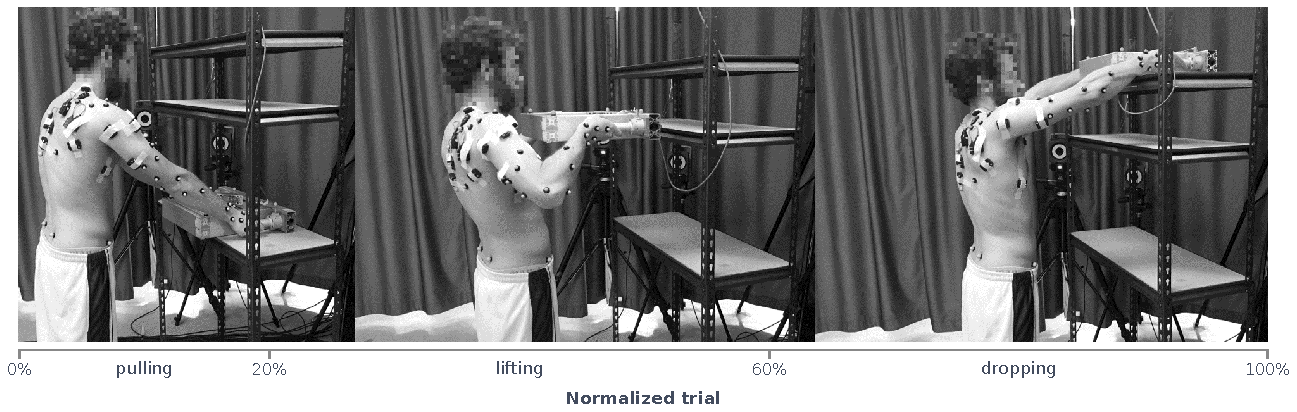
\includegraphics[width=1\linewidth]{fig/phases.pdf}
    \caption{The pulling (from 0 to 20\% of the trial), lifting (21-60\%) and dropping (61-100\%) phases of the lifting task.}
    \label{fig:phases}
\end{figure}

\subsection{Data collection}\label{subsec:data-collection}

The right handle of the box was instrumented with a 6-degree-of-freedom force sensor (Sensix, Poitiers, France) used to measure external forces and define the beginning and the end of each trial.
Markers kinematics were recorded with a VICON™ motion analysis system (Oxford Metrics Ltd, Oxford, UK) and the \citet{Jackson2012-uj} markers model.
Assuming that the left and right sides of the upper body behaved symmetrically during a symmetrical lifting task~\cite{Bouffard2019-fd, Martinez2019-mm, Nielsen1998-fc}, only the right side of the participant was evaluated.

\subsection{Data processing}\label{subsec:data-processing}

All musculoskeletal computations were carried using the OpenSim software API~\cite{Delp2007-ol} and batch processed with the Pyomeca and Pyosim Python libraries~\cite{martinez-pyo}.
The generalized coordinates were computed by inverse kinematics from a custom scaled \citet{Wu2016-kw} upper extremity model (details in~\ref{sec:custom-wu-shoulder-model}).
Then, muscle activations and forces were estimated by static optimization from the generalized coordinates and external forces measured with the instrumented box~\cite{Anderson2001-ma, Erdemir2007-ou}.
These muscle forces were resolved by minimizing the sum of squared muscle activations.
Residual actuators, that account for the non-modelled passive structures~\cite{Hicks2015-wl}, have been added for all joints.
Finally, the glenohumeral joint reaction forces were calculated.
These forces correspond to the internal loads applied on the joint.
The glenohumeral forces were expressed in the local reference frame of the glenoid.
From these forces, we reported the relative time spent beyond a shear-compression dislocation ratio ($\frac{\textrm{shear}}{\textrm{compression}} > 56$\%~\cite{Dickerson2007-qj}).
Three \textsc{ulmd} risk indicators were extracted from this data processing: (1) the sum of muscle activations, (2) the sum of muscle forces and (3) the relative time spent beyond a shear-compression dislocation ratio.

\subsection{Statistics}\label{subsec:statistics}

Time series risk indicators (sum of muscle activations and forces) were time normalized to 1000 data points.
Women and men were then compared using the statistical parametric mapping procedure implemented in the spm1d Python library~\cite{Pataky2010-zh}.
This technique avoids the information loss associated with standard methods which reduce time series into a single, arbitrary, data point (such as mean or median) while controlling for type $\alpha$ error due to multiple comparisons.
Nonparametric testing~\cite{Nichols2002-ri} was chosen as it leads to results qualitatively identical to parametric testing, while being robust to non-normal and non-spherical data~\cite{Pataky2015-ss}.
We tested the main and interaction effects between sex (women \textit{vs} men) and mass (6~kg \textit{vs} 12~kg) on the three \textsc{ulmd} risk indicators with a nonparametric two-way \textsc{anova}.
Each significant difference was reported with the cluster duration, the mean difference, the p-value and the \citet{Cohen2013-tj} $d$ effect size (\textsc{es}).
\textsc{es} was interpreted as large (\textsc{es} $\geq$ 0.8), medium (0.8 $>$ \textsc{es} $\geq$ 0.5) or small (\textsc{es} $<$ 0.5).
While the analyses described above make it possible to analyze time series, statistical inferences were also carried on empirical cumulative distribution functions (\textsc{ecdf}).
The \textsc{ecdf} evaluated at $x$ is defined as the fraction of the points of data which are $\leq x$.
Thus, the \textsc{ecdf} can be graphically represented as the percentile ($x$-axis) associated with each value ($y$-axis).
This method allows exploring distribution objectively, without choosing any parameters as opposed to other techniques (number of binning classes for histograms or bandwidth for kernel density estimation).

    \section{Results}\label{sec:results}
    \subsection{General description}\label{subsec:general-description}

The sum of muscle activations over time during the lifting task is characterized by two peaks (Figure~\ref{fig:general_sum}, left panel).
The first peak ($454 \pm 210$\%~MVC) appears in the middle of the pulling phase (9\% of the trial) while a higher second peak ($694 \pm 343$\%~MVC) appears in the middle of the dropping phase (71\% of the trial).
The sum of muscle forces follows a similar pattern (Figure~\ref{fig:general_sum}, right panel).
A first peak ($1805 \pm 728$~N) occurs in the middle of the pulling phase and a second peak ($2858 \pm 1303$~N) in the middle of the dropping phase.

\begin{figure}[H]
    \centering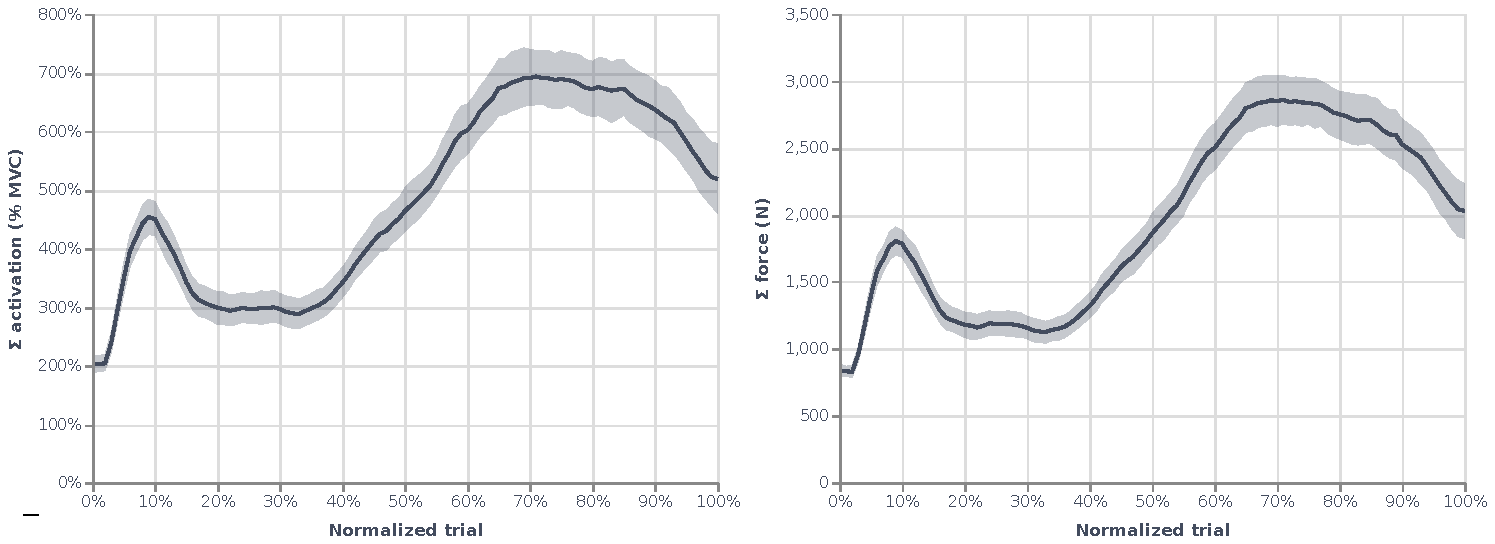
\includegraphics[width=1\linewidth]{fig/sum_general.pdf}
    \caption{Mean (lines) and 95\% confidence interval (areas) of the sum of muscle activations (left panel) and sum of muscle forces (right panel) over time.}
    \label{fig:general_sum}
\end{figure}

With regard to the density of muscle activations of all muscles (Figure~\ref{fig:general_ecdf}, left panel), half of the data is associated with low activation ($1 \pm 0$\%~MVC) while the other half has higher activation ($31 \pm 31$\%~MVC).
About 60\% of the data are below $7 \pm 5$\%~MVC, 80\% of the data are below $35 \pm 23$\%~MVC and 100\% are below $95 \pm 10$~\% MVC\@.
The density of the muscle forces (Figure~\ref{fig:general_ecdf}, right panel) is also delimited by half of the data associated with a low forces ($4 \pm 3$~N) and the other half with higher forces ($125 \pm 149$~N).
About 60\% of the data are below $23 \pm 11$~N, 80\% of the data are below $110 \pm 33$~N and 100\% below $554 \pm 216$~N\@.

\begin{figure}[H]
    \centering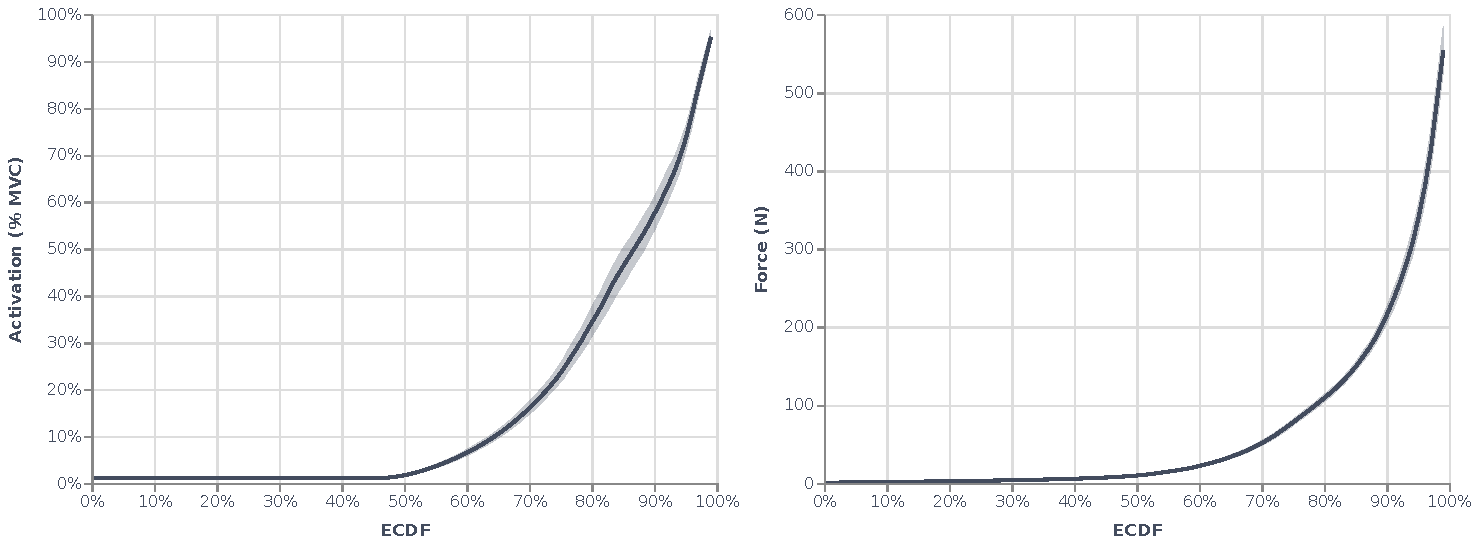
\includegraphics[width=1\linewidth]{fig/ecdf_general.pdf}
    \caption{Mean (lines) and 95\% confidence interval (areas) of the empirical cumulative distribution function (\textsc{ecdf}) of muscle activations (left panel) and muscle forces (right panel).
    The \textsc{ecdf} evaluated at x is defined as the fraction of the data points that are $\leq x$.}
    \label{fig:general_ecdf}
\end{figure}

The distribution of muscle activations (Figure~\ref{fig:dist}, left panel) reveals that several muscles are weakly activated (100\% of the time $<$20\%~MVC), particularly the \textsc{tmaj}, \textsc{tric}, \textsc{pecm}3, \textsc{delt}3, \textsc{pecm}2, \textsc{sbcl}, \textsc{corb}, \textsc{trp}4, \textsc{pmn}.
The five most activated muscles are \textsc{trp}1, \textsc{infsp}, \textsc{delt}1, \textsc{delt}2 and \textsc{trp}2--each with a large activation range (10-80\% MVC).
Similarly, the distribution of muscles forces (Figure~\ref{fig:dist}, right panel) reveals that many muscles are lightly involved (100\% of the time $<$100~N) (\textsc{tmaj}, \textsc{rmj}2, \textsc{sbcl}, \textsc{pecm}3, \textsc{rmj}1, \textsc{pmn}, \textsc{corb}, \textsc{pecm}2, \textsc{delt}3 and \textsc{trp}3) and a similar muscles group with high forces (\textsc{infsp}, \textsc{delt}2, \textsc{delt}1, \textsc{lat}, \textsc{trp}1).

\begin{figure}[H]
    \centering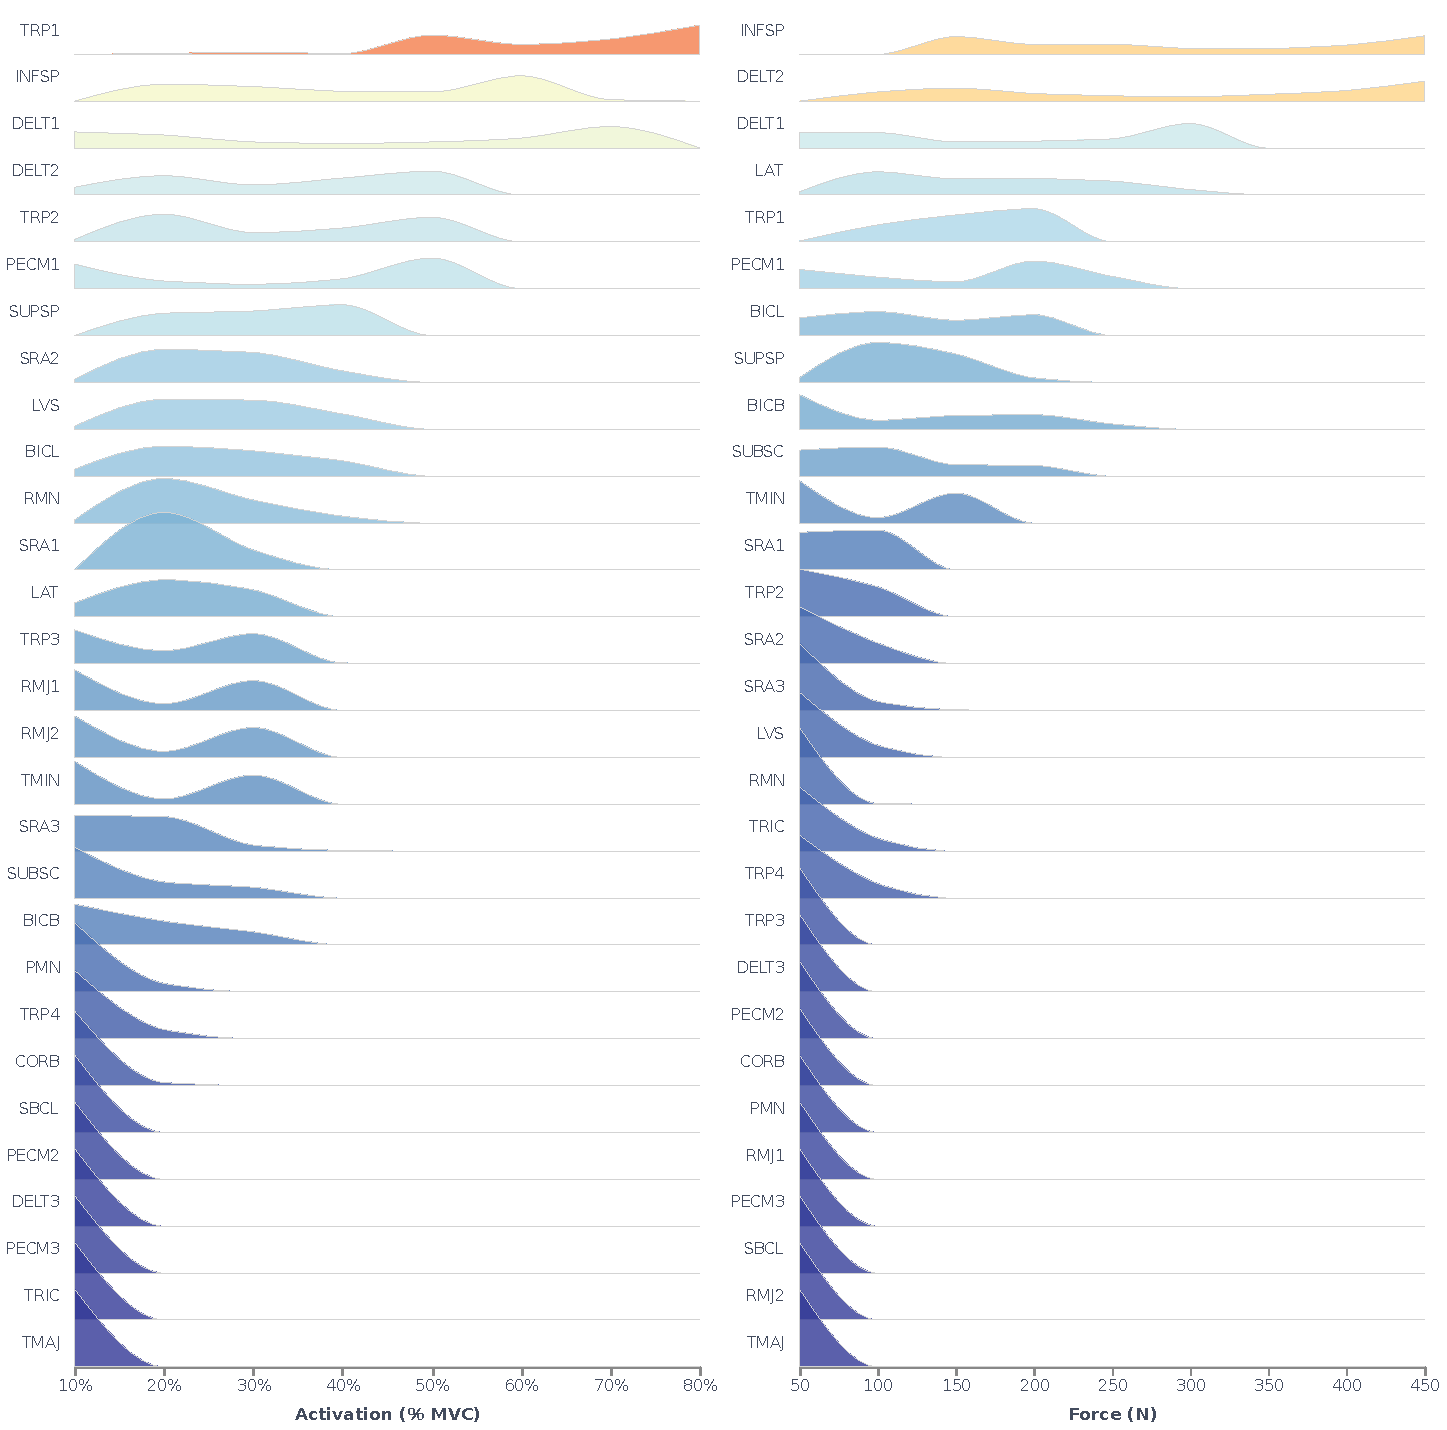
\includegraphics[width=1\linewidth]{fig/dist.pdf}
    \caption{Distribution of muscle activations (left panel) and muscle forces (right panel) for each muscle of the musculoskeletal model.
    The muscles are classified in descending order.
    The distribution is approximated by kernel density estimation and normalized so that the sum of each distribution is equal to 1.
    muscle abbreviations are defined in~\ref{subsec:muscle-abbreviations}}
    \label{fig:dist}
\end{figure}

\subsection{Sex and mass main effects}\label{subsec:sex-and-mass-main-effects}

The sum of muscle activations (Figure~\ref{fig:sum_effects}, top panel) is higher in women during the dropping phase (sex main effect from 55 to 99\%; $+202$\%~MVC; $p<0.001$; $\textrm{ES} = 0.61$ [medium]) and with a 12~kg box during the pulling phase (mass main effect from 8 to 23\%; $+146$\%~MVC; $p<0.001$; $\textrm{ES} = 0.73$ [medium]).
Similarly, the sum of muscle forces (Figure~\ref{fig:sum_effects}, bottom panel) is higher in women during the dropping phase (sex main effect from 77 to 99\%; $+763$~N; $p<0.001$; $\textrm{ES} = 0.59$ [medium]) and with a 12~kg box during the pulling phase (mass main effect from 8 to 24\%; $+535$~N; $p<0.001$; $\textrm{ES} = 0.74$ [medium]).
The 12~kg box also generates higher muscle forces during the dropping phase (mass main effect from 68 to 79\%; $+614$~N; $p = 0.002$; $\textrm{ES} = 0.49$ [small]).

\begin{figure}[H]
    \centering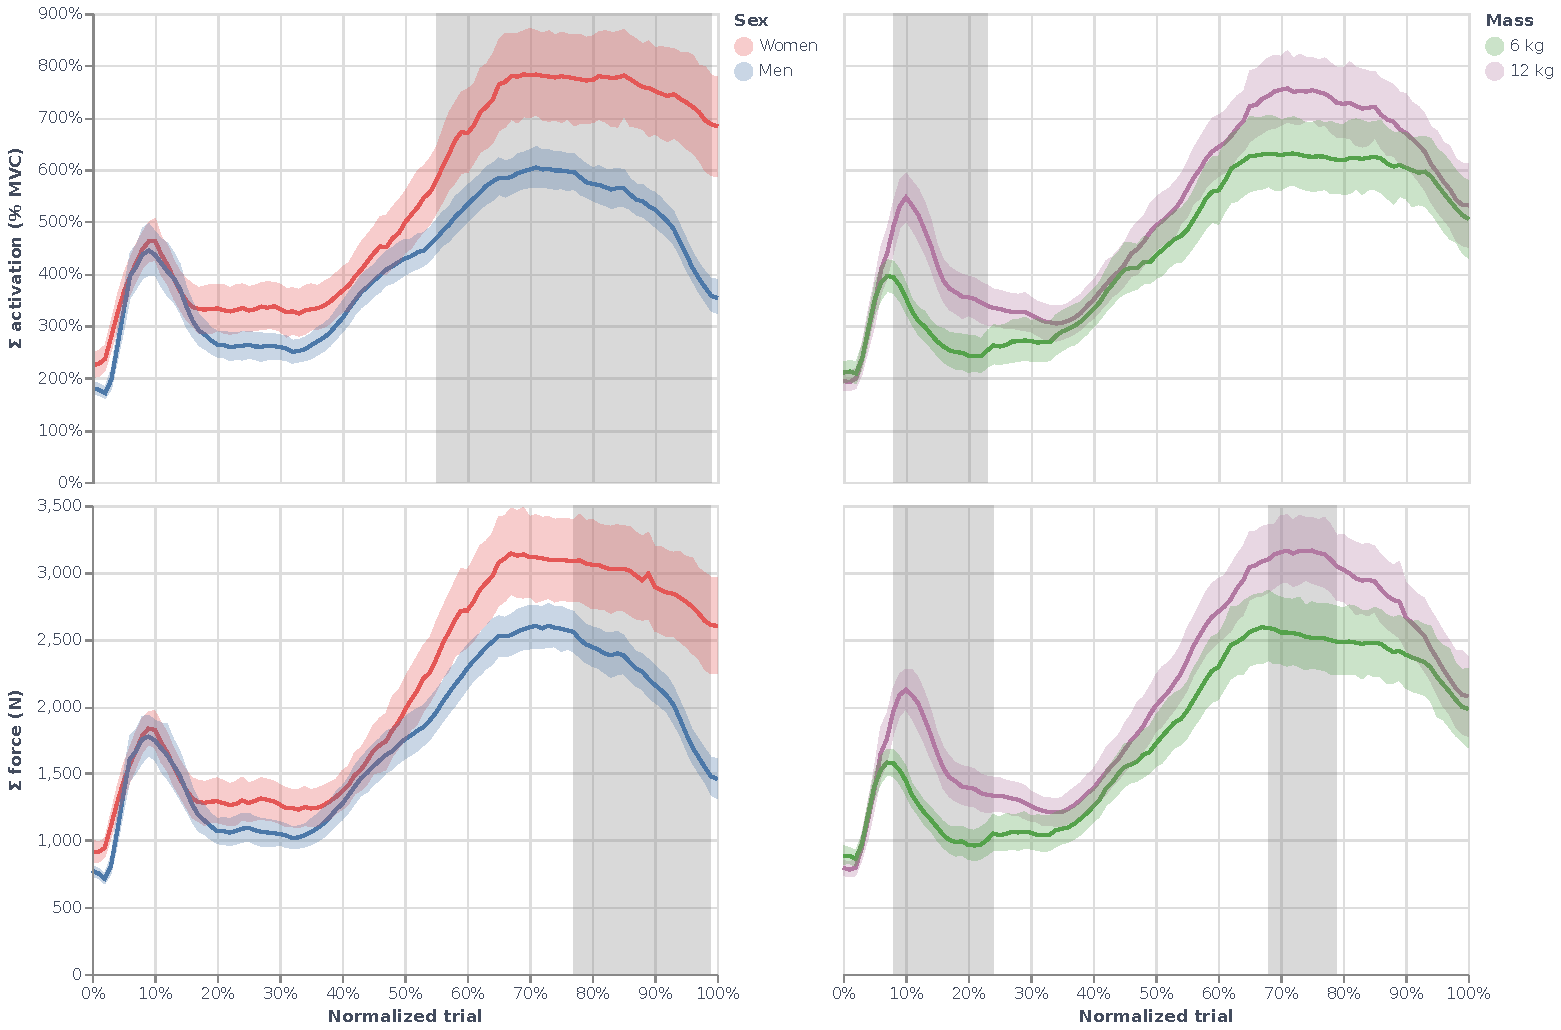
\includegraphics[width=1\linewidth]{fig/sum_effects.pdf}
    \caption{Mean (lines) and 95\% confidence interval (areas) of the sum of muscle activations (upper panels) and sum of muscle forces (lower panels) with the sex (left panel: women in red and men in blue) and mass (right panel: 6~kg in green and 12~kg in purple) main effects.
    A grey area is represented in the presence of a significant effect over time.}
    \label{fig:sum_effects}
\end{figure}

The density of high intensity muscle activations (Figure~\ref{fig:ecdf_effects}, upper panel) is higher in women (sex main effect from 65 to 95\textsuperscript{th} percentiles; $+13$\%~MVC; $p<0.001$; $\textrm{ES} = 0.51$ [medium]) and with a 12~kg box (mass main effect from 90 to 99\textsuperscript{th} percentiles; $+13$\%~MVC; $p<0.001$; $\textrm{ES} = 0.56$ [medium]).
The density of high muscle forces (Figure~\ref{fig:ecdf_effects}, bottom panel) is also higher in women (sex main effect from 58 to 80\textsuperscript{th} percentiles; $+10$~N; $p = 0.001$; $\textrm{ES} = 0.39$ [small] and from 88 to 99\textsuperscript{th} percentiles; $+68$~N; $p = 0.002$; $\textrm{ES} = 0.44$ [small]) and with a 12~kg box (mass main effect from 67 to 97\textsuperscript{th} percentiles; $+27$~N; $p < 0.001$; $\textrm{ES} = 0.24$ [small]).

\begin{figure}[H]
    \centering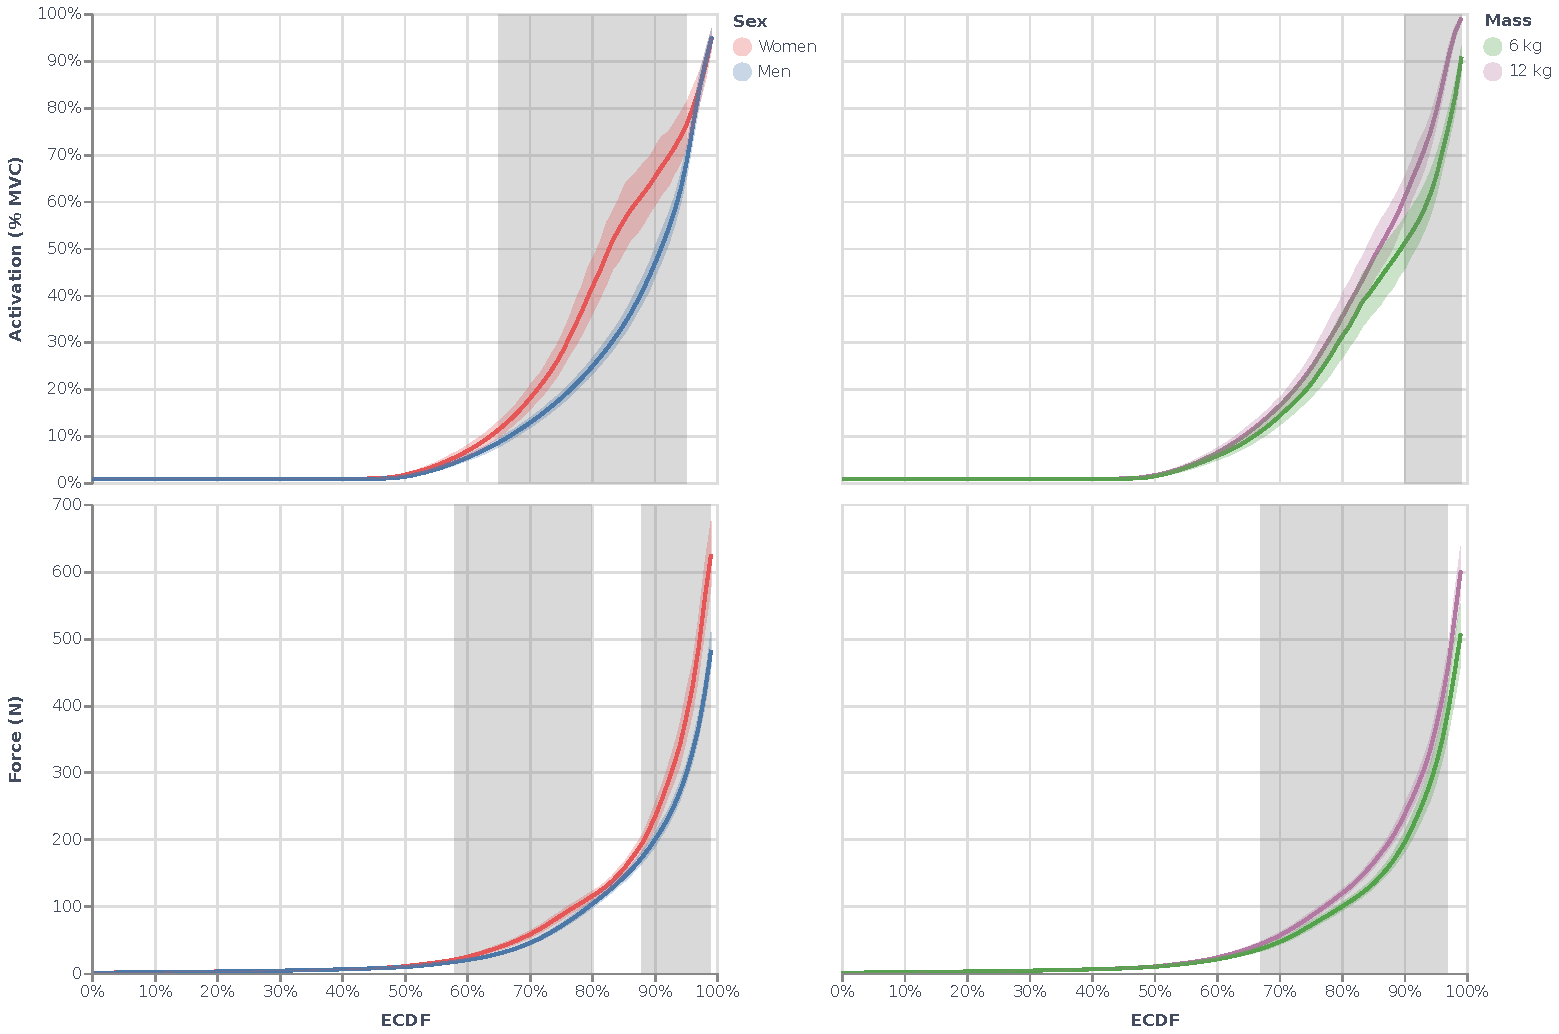
\includegraphics[width=1\linewidth]{fig/ecdf_effects.pdf}
    \caption{Mean (lines) and 95\% confidence interval (areas) of the empirical cumulative distribution function (\textsc{ecdf}) of muscle activations (upper panels) and muscle forces (lower panels) with the sex (left panels: women in red and men in blue) and mass (right panels: 6~kg in green and 12~kg in purple) main effects.
    The \textsc{ecdf} evaluated at $x$ is defined as the fraction of the data points that are $\leq x$.
    A grey area is represented in the presence of a significant effect.}
    \label{fig:ecdf_effects}
\end{figure}

The relative time spent beyond a shear-compression dislocation ratio (Figure~\ref{fig:dislocation}) is higher in women (sex main effect; $+5$\%; $p = 0.045$; $\textrm{ES} = 0.29$ [small]) and remains constant between 6 and 12~kg (no mass main effect).

\begin{figure}[H]
    \centering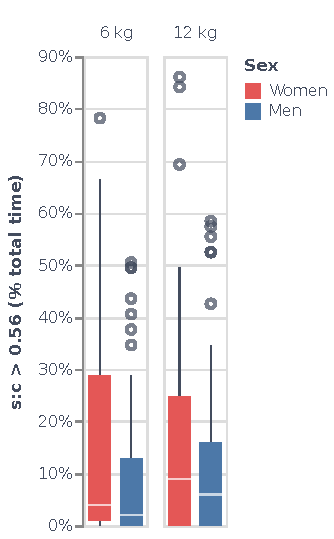
\includegraphics[width=0.3\linewidth]{fig/dislocation.pdf}
    \caption{Boxplot of the relative time spent beyond a shear-compression dislocation ratio by sex (women in red and men in blue) and mass (6~kg on the left panel and 12~kg on the right panel) with median (horizontal lines), first-third interquartile range (bars), first-third interquartile range multiplied by 1.5 times the interquartile difference [$\textrm{Q1} - 1.5 \times \textrm{IQR}; \textrm{Q2} + 1.5 \times \textrm{IQR}$] (vertical lines).
    Data beyond the end of the whiskers are considered outliers (points).}
    \label{fig:dislocation}
\end{figure}

    \section{Discussion}\label{sec:discussion}
    In this study, we investigated the sex and mass effects on three musculoskeletal indicators when women and men lifted 6~kg and 12~kg boxes from hip to eye level.
As hypothesized, women generated more muscle force and activation than men, regardless of the mass lifted.
Those differences occurred during the dropping phase, when the box was above shoulder level.
In addition, women appear to spent more time beyond a shear-compression dislocation ratio.

\subsection{General profile of muscle forces and activations}\label{subsec:general-profile-of-muscle-forces-and-activations}

As previously reported in electromyography~\cite{Bouffard2019-fd}, our results show that participants generated two distinct peaks of muscle forces and activations during the pulling and dropping phases.
Those two peaks appear when the box is the furthest from the trunk (\ref{sec:box-thorax-distance-and-hip-displacement}) leading to a longer--ineffective--lever arm which decreases the mechanical efficiency of the lift.
The second peak reached a higher force and activation amplitude, probably due to elongated muscle lever arms when participants lifted the box higher, which requires more muscle activation to stabilize the upper limb.
As the muscle force and activation increase with the box height, the risk of upper limb injury is also likely to increase~\cite{Blache2015-oc}.
A wide range of studies already pointed out that exposure to above-shoulder work contributes to degenerative damage to the rotator cuff (see \citet{Van_der_Molen2017-sb} for a review) and should be avoided.
Similarly and as expected, a heavier box generates higher musculoskeletal stresses when the box is the furthest from the trunk.
This is in accordance with the literature~\cite{Blache2015-xe, Yoon2012-ap} and our electromyographic study~\cite{Bouffard2019-fd} and suggest lifting lighter boxes to avoid \textsc{ulmd}s.

The anterior and lateral deltoids are the prime movers during box lifting tasks~\cite{Blache2017-pv,Blache2015-oc,Bouffard2019-fd}.
Our results show that these muscles are highly solicited, in terms of muscle force and activation.
In agreement with \citet{Blache2015-oc}, the upper trapezius and infraspinatus also showed high forces and activations.
These muscles participate in arm elevation~\cite{Ackland2008-vt, Escamilla2009-ho} and their contribution increases with the lifting height~\cite{Blache2015-oc, Herberts1984-xk}.
Although we expected for antagonists (e.g., posterior deltoid, triceps brachii) and stabilizing (e.g., coracobrachialis, teres major) muscles to be less activated than agonists, our results show that the contribution of these muscles is almost null.
The static optimization cost function--which minimize the sum of squared muscle activations--is well known to neglect the stabilization and coactivation components~\cite{Gottlieb2000-ga, Kian2019-gz} and could explain why half of our data points are close to zero.

\subsection{Kinematic, electromyographic and musculoskeletal evidences of the sex-related differences}\label{subsec:kinematic,-electromyographic-and-musculoskeletal-evidences-of-the-sex-related-differences}

The physiological differences between women and men are well documented (see \citet{Cote2012-hn} for a review) and result with women’s lifting strength ranging between 40 and 70\% of men’s \citet{Kumar2004-fv}.
For a given load, women are thus closer to their maximum capacity than men.
While the kinematic differences reported in \citet{Martinez2019-mm} depend on the mass lifted by women, no sex-mass interaction was reported in \citet{Bouffard2019-fd} and in this study.
For any men-women mass ratio (100\%: 6--6~kg and 12--12~kg;
50\%: 6--12~kg), women still have higher \textsc{emg}~\cite{Bouffard2019-fd}, muscle forces and muscle activations.
This suggests that, either a 50\% mass reduction is not sufficient to control for strength differences, or that strength alone does not explain the musculoskeletal differences.
If the first suggestion is proven, acceptable weights should be reviewed as it would be expected that 90\% of women would be able to safely lift a 12~kg box from hip to eye level twice every minute for an 8-hour shift~\cite{Waters1993-nk,Waters2016-lw}.
The second suggestion seems more plausible--while strength alone does not explain EMG and musculoskeletal differences, the kinematics adaptations in response to a different box mass-strength ratio could.
Women would compensate for their strength deficits with a safe technique, but surprisingly the opposite happens and in a different way depending on the box mass.
We showed that women use more the glenohumeral joint~\cite{Martinez2019-mm} and keep the box further from the trunk (\ref{sec:box-thorax-distance-and-hip-displacement}) to lift a 6~kg box compared to men.
In addition to increasing loading on the spine~\cite{Marras2006-jq}, this technique could also increase forces located at the shoulder joint during extreme range of motion~\cite{Kim2003-lf}.
An increase in the mass to lift can change coordination to reduce the amount of muscle effort required~\cite{Burgess-Limerick1995-uh}, but still women use their lower limbs less than men to lift a 12~kg box (\ref{sec:box-thorax-distance-and-hip-displacement}).
By taking more contribution to the box height, the use of lower limbs could reduce shoulder stress~\cite{Kim2003-lf}.
Thus, men would systematically use a safer technique than women for all the weights we considered, which could explain why women have higher musculoskeletal loads in our study.

It seems unlikely that the kinematic alterations just described do not lead to a different muscle coordination scheme.
During the experimental task, women indeed generated a higher sum of muscle activations and forces than men during the dropping phase.
\citet{Bouffard2019-fd} also reported higher muscle activation in women, particularly for prime movers.
While both studies have specific limitations, they both point to similar conclusions.
In both studies, the muscle activation in the 90\textsuperscript{th} percentile reached by women seems to be a major muscular effort to be maintained in professional settings (around 65\% MVC in women against 50\% MVC in men).

We have also shown that women might spend more time with a high risk of humerus dislocation.
A greater muscle activation, muscle force and glenohumeral contribution during the handling task will indeed increase the solicitation of passive structures and alter the glenohumeral stability~\cite{Bergmann2007-zj}.
This high ratio of shear and compression forces imposes high stresses on the stabilizing muscles and thus increases the risk of developing \textsc{ulmd}.
The infraspinatus, anterior deltoid and lateral deltoid muscles are all three stabilizers of the humerus~\cite{Blache2017-pv, Yanagawa2008-es} and are also the muscles with the highest sum of muscle forces in our dataset.
This underlines the importance of strengthening those muscles for manual handling workers to maintain shoulder stability and avoid injuries~\cite{Sharkey1995-gl}.

Women generally work more often and for a longer time than men in an overhead position~\cite{Dahlberg2004-mw}.
The sex-related differences reported in our three studies occurred mainly in this position, which is considered a risk factor for shoulder injuries~\cite{Antony2010-ji, Dal_Maso2016-ol, Grieve2008-je} and the leading cause of rotator cuff tear~\cite{Palmerud2000-mp, Vecchio1995-ke}.

As a summary, our previous works in kinematics~\cite{Martinez2019-mm} and electromyography~\cite{Bouffard2019-fd} showcased sex-related differences during a box lifting task.
In this study, we found evidence of a sex effect on musculoskeletal indicators.
These three categories of indicators are, by definition, dependent on each other.
Taken together, however, they do provide an overview of the complex interaction between biomechanical variables that could explain the higher prevalence of ULMD among women (Figure~\ref{fig:links}).
This interaction starts with the biological differences mentioned in \citet{Cote2012-hn}.
Women would compensate for these biological differences by altering their lifting technique, as reported in~\cite{Martinez2019-mm}.
These kinematic differences will then influence muscle activations, reported in~\cite{Bouffard2019-fd}, and the musculoskeletal loads mentioned in this study.
Greater musculoskeletal loads--in addition to unobserved factors--may explain the higher prevalence of upper limb injury in women.

\begin{figure}[H]
    \centering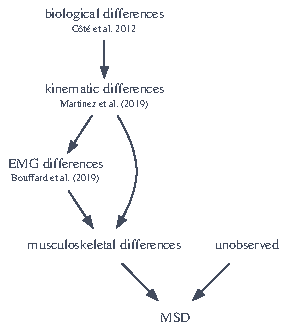
\includegraphics[width=0.5\linewidth]{fig/links.pdf}
    \caption{Conceptual framework to link the biomechanical evidences underlying the sex-related differences in the prevalence of upper limb \textsc{ulmd}.}
    \label{fig:links}
\end{figure}

\subsection{Methodological considerations}\label{subsec:methodological-considerations}

To properly interpret the results of this study, it is necessary to consider some methodological points concerning the experimental task, the scaling of the musculoskeletal model and the static optimization.
First, we designed the experimental task to control for sex effect on deposit height (shelf adjusted at eye level) and box mass (6 and 12~kg).
We showed a sex main effect regardless of the mass.
It would be preferable to measure the maximum strength of each participant and adjust the box mass accordingly to control for strength effect on our variables.
Second, many simplifying hypotheses are required when creating a musculoskeletal model, whether on muscle parameters or on muscle forces distribution to solve muscle redundancy.
One of the first limitations comes from the validation of the muscle trajectories of the \citet{Wu2016-kw} model performed on simple movements compared to our complex handling task.
In addition, the use of a generic model does not allow the musculoskeletal parameters to be personalized for each participant.
As a result, inter-individual variability is reduced and the activation or strength of certain muscles may be overestimated.
The adaptation of a musculoskeletal model to various populations and to a task above the shoulders involved many technical challenges, particularly in terms of muscle trajectories (\ref{sec:custom-wu-shoulder-model}).
Despite the above limitations, few biomechanical, ergonomic or musculoskeletal studies include so many participants from specific populations ($n = 40$).
Third, muscle forces and activations estimated from static optimization can be influenced by several factors such as the cost function, the model parameters and the joint kinematics~\cite{Bolsterlee2013-ij, Gottlieb2000-ga}.
The main limitation of our static optimization is that it does not consider muscle co-activation with a least square cost function~\cite{Kian2019-gz}.
Several solutions exist to obtain physiological activations.
The implementation of a non-dislocation constraint on the humerus~\cite{Blache2017-pv} to ensure that the balance of muscular forces is oriented towards the glenoid, the tracking of \textsc{emg} signals~\cite{Pizzolato2015-gm} or a direct dynamic approach with \textsc{emg} signals tracking~\cite{Belaise2018-wo} are some of them.
\citet{Bouffard2019-fd} have shown that sex has no effect on glenohumeral muscle co-activation, which nuances the need to include co-activation in the study of sex-related differences during a lifting task.

\subsection{Implications}\label{subsec:implications}

Work-related musculoskeletal injury is a complex multi-causal phenomenon.
Our results suggest a careful consideration of sex during ergonomic interventions on overhead tasks.
With our work on kinematics, electromyography and musculoskeletal modelling, we developed new biomechanical \textsc{ulmd} risk indicators.
The development of synthetic indicators is a step towards objective quantification of exposure to physical risk factors.
They can be used to evaluate a particular work task or technique and estimate the underlying musculoskeletal loads.
They are, for example, already applied in ergonomics investigation to report the expertise-related difference during a lifting task~\cite{goubault-evsn}.
In our case, these synthetic indicators reinforced known recommendations and emphasized the importance of a proper lifting technique on musculoskeletal loads and by extension \textsc{ulmd} prevalence.
In order to mitigate the musculoskeletal loads on the upper limb during a lifting task, we recommend a technique that keeps the box closer from the trunk, reduces above shoulder work, makes greater use of the lower limbs and reduces the glenohumeral joint contribution.
Practitioners may also consider adapting the work environment to include lighter boxes, stabilizing muscle strengthening sessions and more generally physical activity to improve muscle strength and endurance.
These incentives are particularly recommended for female workers to compensate for the strength differential compared to men.
Taken together, our studies on kinematics~\citep{Martinez2019-mm}, \textsc{emg}~\citep{Bouffard2019-fd} and musculoskeletal biomechanics suggest that it is crucial for practitioners to give a special attention to women during above-shoulder work.
Our indicators show that the biomechanical loads are higher in women compared to men while working above shoulder, which is critical for the development of shoulder injury~\citep{Van_der_Molen2017-sb}.
It would therefore be necessary to adapt workload in women working in such position.
Beyond sex-related differences, we defend an ergonomic practice based on a process tailored to each worker and based on multidisciplinary scientific works.

    \section{Acknowledgements}\label{sec:acknowledgements}

    The study was financially supported by the Institut de Recherche Robert-Sauvé en Santé et Sécurité du Travail [\# 2014--0045].
    The authors would like to thank the workers who participated as well as Marjolaine Corbeil, Landry Desmoulins and Damien Leflem for their contribution during the data collection and data labelling.

    \appendix
    \section{Custom Wu shoulder model}
\label{sec:custom-wu-shoulder-model}

\subsection{Arm muscles}\label{subsec:arm-muscles}

Two lines of action for the biceps brachii, and the long head of the triceps brachii were added to the model to account for the contribution of the arm muscles to the glenohumeral joint.

\subsection{Wrapping objects}\label{subsec:wrapping-objects}

We modified the wrapping objects to avoid sudden changes in muscle trajectories, lighten the model and duplicate objects to prevent using a single object for several muscles.
Wrapping object dimensions were modified as needed while preserving the muscles lengths.
The active quadrants of the wrapping objects have been identified to reduce singular points.
Ellipsoidal objects have been reduced to a minimum, and replaced by cylindrical objects.
This change should reduce the computation time, without influencing the trajectories for our range of motion.

\subsection{Muscle lengths}
\label{subsec:muscle-lengths}

We modified the normalized muscle lengths to maintain them within a physiological range $[0.5;1.5]$.
We analysed muscle lengths during high amplitude trials for all participants to identify muscles with low (generation of minimal effort) or high (high passive force) lengths.
The normalized lengths of these muscles have been modified by changing the optimal fiber lengths and/or changing the dimensions of the wrapping objects.
The modifications were made, while respecting the initial values of the lever arms of each muscle with respect to each degree of freedom.
The modified muscles are the anterior serratus anterior, the rhomboid and the pectoralis minor.

\subsection{Muscle abbreviations}\label{subsec:muscle-abbreviations}

\textsc{bicb}: biceps brachii short head

\textsc{bicl}: biceps brachii long head

\textsc{corb}: coracobrachialis

\textsc{delt}1: anterior deltoid

\textsc{delt}2: medial deltoid

\textsc{delt}3: posterior deltoid

\textsc{infsp}: infraspinatus

\textsc{lat}: latissimus dorsi

\textsc{lvs}: levator scapulae

\textsc{pecm}1: pectoralis major superior

\textsc{pecm}2: pectoralis major medial

\textsc{pecm}3: pectoralis major inferior

\textsc{pmn}: pectoralis minor

\textsc{rmj}1: rhomboid major superior

\textsc{rmj}2: rhomboid major inferior

\textsc{rmn}: rhomboid minor

\textsc{sbcl}: subclavius

\textsc{sra}1: serratus anterior superior

\textsc{sra}2: serratus anterior medial

\textsc{sra}3: serratus anterior inferior

\textsc{subs}: subscapularis

\textsc{supsp}: supraspinatus

\textsc{tmaj}: teres major

\textsc{tmin}: teres minor

\textsc{tric}: triceps brachii

\textsc{trp}1: upper trapezius

\textsc{trp}2: middle trapezius superior

\textsc{trp}3: middle trapezius inferior

\textsc{trp}4: lower trapezius

\section{Box-thorax distance and hip displacement}\label{sec:box-thorax-distance-and-hip-displacement}


\begin{figure}[H]
    \centering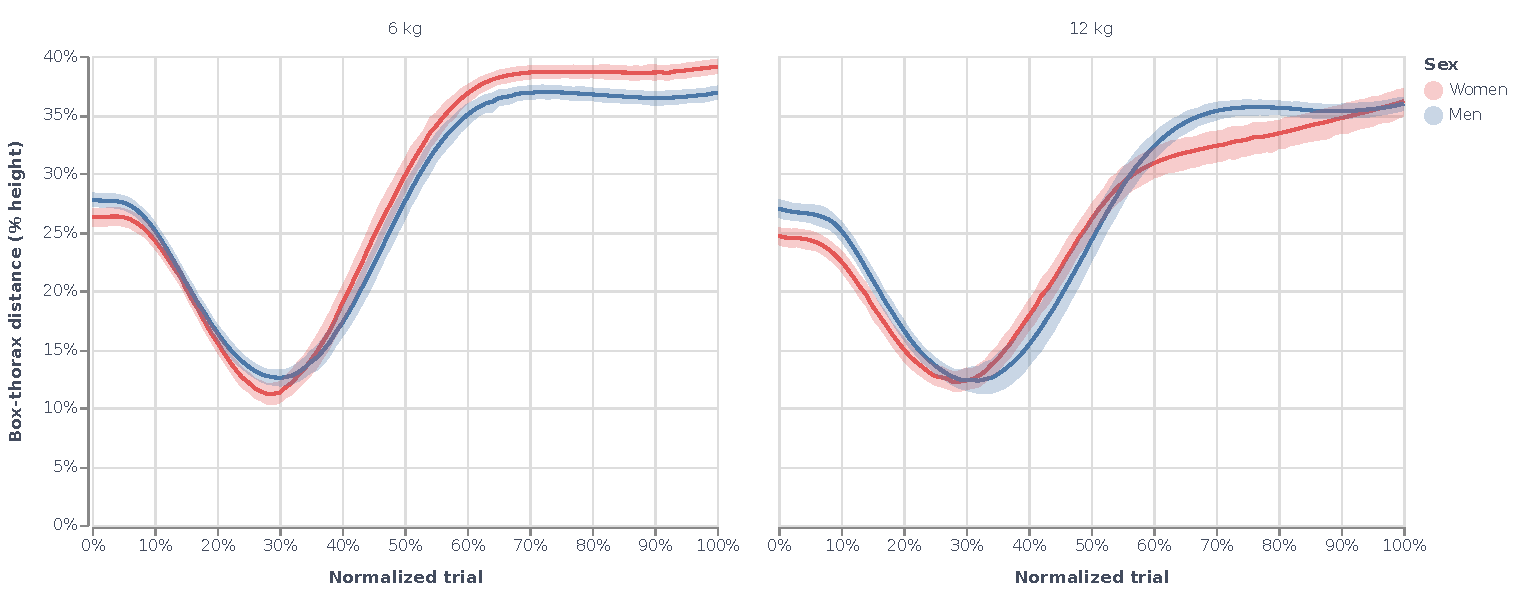
\includegraphics[width=1\linewidth]{fig/box-thorax.pdf}
    \caption{Mean (lines) and 95\% confidence interval (areas) of the box-thorax distance expressed in percentage of the participant's height by sex (women in red and men in blue) with a 6~kg (left panel) and 12~kg (right panel) box.}
\end{figure}

\begin{figure}[H]
    \centering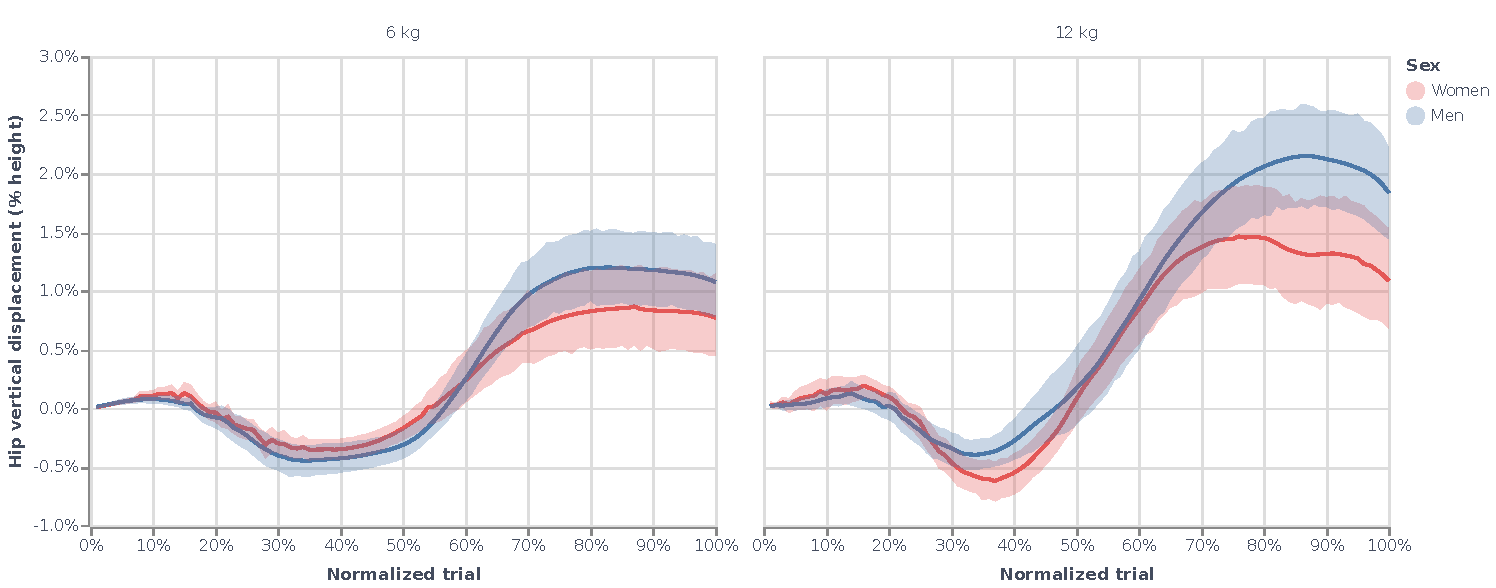
\includegraphics[width=1\linewidth]{fig/hip-displacement.pdf}
    \caption{Mean (lines) and 95\% confidence interval (areas) of the hip vertical displacement distance expressed in percentage of the participant's height by sex (women in red and men in blue) with a 6~kg (left panel) and 12~kg (right panel) box.}
\end{figure}



    \bibliographystyle{elsarticle-num-names}
    \bibliography{ref}

\end{document}